%!TEX TS-program = pdflatexmk

% Copyright (c) 2018 - 2022, Martin Scheidt (ISC license)
% Permission to use, copy, modify, and/or distribute this file for any purpose with or without fee is hereby granted, provided that the above copyright notice and this permission notice appear in all copies.

\documentclass[border=2]{standalone}

\usepackage[dev]{tikz-trackschematic}

\begin{document}
  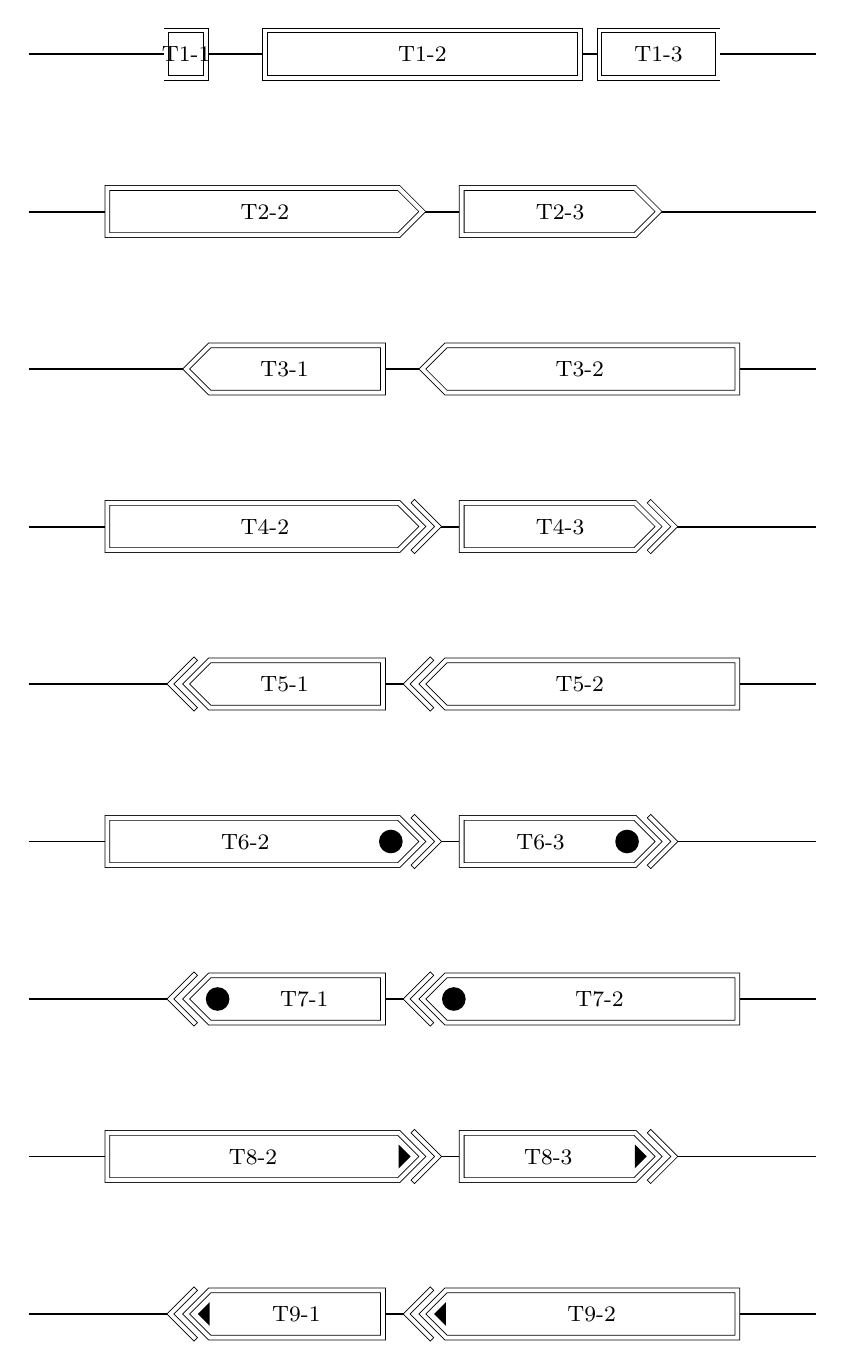
\begin{tikzpicture}
  
    \foreach \i in {1,2,...,9}{% base coordinate
      \coordinate (A\i) at ($(-1,0) + 2*(0,-\i)$);
      \coordinate (B\i) at ($( 9,0) + 2*(0,-\i)$);
    }

    \foreach \i in {1,2,...,9}{% draw main tracks on base coordinate
      \secondarytrack (A\i) --   (B\i);
    }

    \foreach \i in {1,2,...,9}{% coordinates for testing symbols
      \coordinate (T\i-1) at ($(1,0) + 2*(0,-\i)$);
      \coordinate (T\i-2) at ($(4,0) + 2*(0,-\i)$);
      \coordinate (T\i-3) at ($(7,0) + 2*(0,-\i)$);
    }

    \parkedvehicles[length=0.5cm] at (T1-1) label (T1-1);
    \parkedvehicles[]             at (T1-2) label (T1-2);
    \parkedvehicles[length=1.5cm] at (T1-3) label (T1-3);

    \shunting[forward]               at (T2-2) label (T2-2);
    \shunting[forward ,length=2.5cm] at (T2-3) label (T2-3);
    \shunting[backward,length=2.5cm] at (T3-1) label (T3-1);
    \shunting[backward]              at (T3-2) label (T3-2);

    \shunting[movement,forward]               at (T4-2) label (T4-2);
    \shunting[movement,forward ,length=2.5cm] at (T4-3) label (T4-3);
    \shunting[movement,backward,length=2.5cm] at (T5-1) label (T5-1);
    \shunting[movement,backward]              at (T5-2) label (T5-2);

    \shunting[operation=manual,movement,forward]               at (T6-2) label (T6-2);
    \shunting[operation=manual,movement,forward ,length=2.5cm] at (T6-3) label (T6-3);
    \shunting[operation=manual,movement,backward,length=2.5cm] at (T7-1) label (T7-1);
    \shunting[operation=manual,movement,backward]              at (T7-2) label (T7-2);

    \shunting[operation=automatic,movement,forward]               at (T8-2) label (T8-2);
    \shunting[operation=automatic,movement,forward ,length=2.5cm] at (T8-3) label (T8-3);
    \shunting[operation=automatic,movement,backward,length=2.5cm] at (T9-1) label (T9-1);
    \shunting[operation=automatic,movement,backward]              at (T9-2) label (T9-2);

  \end{tikzpicture}
\end{document}